
This layer is active when the user is logged in to the app and wants to search for the item in the inventory. Search layer is presented with option of entering item description manually or entering the description using QR reader.This layer helps to find the shelf where the item is stored and to see if the inventory has more of the item searched.
\subsection{Item Description}
This SubSystem deals with the searching the item the inventory has. It will take the input through text input or barcode reader or even the camera.

\begin{figure}[h!]
	\centering
 	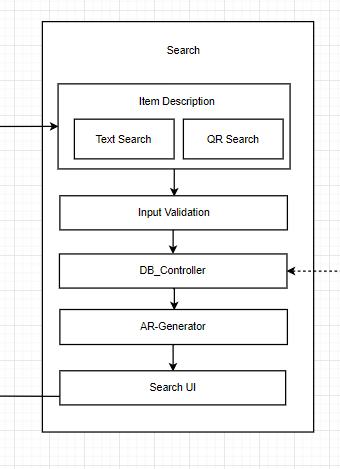
\includegraphics[width=0.60\textwidth]{images/Capture}
 \caption{Example subsystem description diagram}
\end{figure}

\subsubsection{Assumptions}
Here are some assumptions that are made:
\begin{itemize}
    \item The user is logged into the system. 
    \item 
    \item
\end{itemize}

\subsubsection{Responsibilities}


\subsubsection{Subsystem Interfaces}
Each of the inputs and outputs for the subsystem are defined here. Create a table with an entry for each labelled interface that connects to this subsystem. For each entry, describe any incoming and outgoing data elements will pass through this interface.

\begin {table}[H]
\caption {Subsystem interfaces} 
\begin{center}
    \begin{tabular}{ | p{1cm} | p{6cm} | p{3cm} | p{3cm} |}
    \hline
    ID & Description & Inputs & Outputs \\ \hline
    \#xx & Description of the interface/bus & \pbox{3cm}{input 1 \\ input 2} & \pbox{3cm}{output 1}  \\ \hline
    \#xx & Description of the interface/bus & \pbox{3cm}{N/A} & \pbox{3cm}{output 1}  \\ \hline
    \end{tabular}
\end{center}
\end{table}

\subsection{Subsystem 2}
Repeat for each subsystem

\subsection{Subsystem 3}
Repeat for each subsystem

